\documentclass[a4paper]{cas-sc}

\makeatletter
\def\ps@twosidesectiontitlepage{%
   \def\@oddfoot{\hfil\footnotesize Preprint submitted to Elsevier\hfil}%
   \def\@evenfoot{\hfil\footnotesize Preprint submitted to Elsevier\hfil}%
   \def\@oddhead{}%
   \def\@evenhead{}%
}
\renewcommand{\printorcid}{}
\makeatother

\makeatletter
\let\ps@first\ps@plain
\let\ps@cas\ps@plain
\makeatother

\usepackage{hyperref}
\usepackage{amsmath,amssymb,amsfonts}
\usepackage{booktabs}
\usepackage{graphicx}
\usepackage{multirow}
\usepackage{xcolor}
\usepackage{subcaption}
\usepackage{natbib}
\usepackage[pagewise]{lineno}
\usepackage{float}
\restylefloat{table}

%% Convenience commands
\newcommand{\causalfixed}{y^{\mathrm{cf}}}
\newcommand{\fullnr}{y^{\mathrm{nr}}}
\newcommand{\obstime}{t^{\mathrm{obs}}}

%% ─────────────────────────────────────────────────────────────
\begin{document}

\title{Traffic Speed Forecasting Under Nonrecurrent Conditions:
       A Causally-Stratified Large-Scale Benchmark}
\shortauthors{Andrew J. Bae}

\author[1]{Andrew J. Bae\cormark[1]}
\ead{abae@andrew.cmu.edu}
\credit{Conceptualization, Data Curation, Software, Methodology,
        Formal Analysis, Writing -- Original Draft,
        Writing -- Review \& Editing}

\address[1]{Department of Civil and Environmental Engineering,
            Carnegie Mellon University, Pittsburgh, PA, USA}
\cortext[1]{Corresponding author}

% ── Abstract ──────────────────────────────────────────────────
\begin{abstract}
Traffic forecasting models are increasingly evaluated on standard
benchmarks that report aggregate mean absolute error~(MAE) over all
links and timesteps.
Nonrecurrent~(NR) disruptions (crashes, work zones, weather events,
and irregular demand surges) occupy a small fraction of these samples
but account for a disproportionate share of operational delay and are
precisely the conditions where prediction errors matter most.
We present a large-scale empirical benchmark of speed
forecasting performance under NR conditions using fine-grained,
causally grounded per-link, per-timestep stratification.
A key methodological contribution is the \emph{causal observability
framework}: because traffic-state-based NR detection requires three
consecutive flagged intervals (15~min) to confirm a disturbance, the
first two intervals of every NR episode are unobservable at real-time
prediction time.
We formally partition the evaluation into three informationally
distinct regimes, namely \emph{recurrent}, \emph{unobserved onset},
and \emph{confirmed NR}, and show that conflating them conceals the
hardest and most operationally relevant failure mode.
Across 17 models spanning four families (statistical, machine learning,
per-link deep learning, and spatiotemporal graph networks), two
freeway networks (TSMO, Maryland; Cranberry, Pennsylvania), and four
training strategies (standard, weighted loss, NR fine-tuning, and
multi-objective), we find: (1)~NR MAE is 2--5$\times$ higher than
recurrent MAE across all models and both networks; (2)~unobserved
onset MAE substantially exceeds confirmed NR MAE, identifying onset
as the dominant failure mode; (3)~model rankings shift under NR
evaluation relative to aggregate evaluation, with simpler models
competitive with complex graph networks in the onset regime; and
(4)~NR-aware training strategies and richer input features improve
NR performance modestly but do not close the gap with recurrent
performance.
These findings replicate across both networks.
The results call for regime-stratified reporting as a standard
practice in traffic forecasting evaluation and provide a
reproducible baseline for future NR-aware model development.
\end{abstract}

\begin{keywords}
Nonrecurrent congestion \sep
Traffic speed forecasting \sep
Regime-stratified evaluation \sep
Causal observability \sep
Spatiotemporal graph networks \sep
Benchmark
\end{keywords}

\maketitle

\linenumbers

% ══════════════════════════════════════════════════════════════
\section{Introduction}
\label{sec:introduction}
% ══════════════════════════════════════════════════════════════

Freeway traffic is commonly decomposed into a \emph{recurrent} component
(predictable congestion arising from stable demand patterns at known
bottlenecks) and a \emph{nonrecurrent} (NR) component driven by
incidents, work zones, adverse weather, and irregular demand surges
\citep{skabardonis2003, schrank2021, fhwa2025}.
Although NR episodes occupy only 2--5\% of link-timestep observations
on a typical freeway network~\citep{bae2026labeling}, they account for
a disproportionate share of total delay and are the conditions where
prediction errors carry the highest operational cost.
Countermeasures (routing diversions, ramp metering adjustments, and
variable message sign activations) require 5--15~minutes of lead time~\citep{fhwa2025, williams2007tmcsurvey};
a model that fails during onset provides no actionable signal.

The traffic forecasting literature has produced a succession of increasingly
sophisticated spatiotemporal architectures, with several models achieving
mean absolute error (MAE) below 3~mph on standard urban benchmarks
\citep{li2018dcrnn, wu2019gwnet, liu2024largest, shaygan2022survey}.
Yet nearly all published evaluations report a single aggregate error
averaged over all links and timesteps without distinguishing NR from
recurrent periods~\citep{bae2026why}.
Because NR episodes are rare, aggregate MAE is dominated by routine
conditions where recurrent structure is strong and easy to exploit.
A model can improve aggregate MAE while remaining entirely unreliable
during disruptions, and model rankings can appear stable even when
NR-specific performance differs substantially across architectures.

Prior work has identified this gap conceptually and in specific task
settings.
\citet{bae2026why} synthesize the mechanisms by which aggregate
benchmarking masks NR failures in forecasting; \citet{bae2026onset}
demonstrate that standard binary anomaly prediction benchmarks
systematically overstate early-warning performance due to conflation
of episode onset with persistence in the binary positive class.
Neither study provides an empirical benchmark of continuous speed
regression under NR conditions at scale.

The present paper fills this gap with three specific contributions
beyond the prior literature.

\paragraph{Causal observability framework.}
The NR labels used in this study are produced by an ensemble
detector~\citep{bae2026labeling} that requires three consecutive
below-threshold intervals (15~min) before confirming a disturbance.
This confirmation delay is operationally realistic, since real-time
detection systems cannot label an episode until it is confirmed, but
it creates an important informational asymmetry: the first two
intervals of every NR episode are labeled in hindsight but were
not observable at prediction time.
We formalize this as the \emph{causal observability problem} and
introduce three informationally distinct evaluation regimes:
\textbf{recurrent} (no NR signal in context or target),
\textbf{unobserved onset} (NR in target, but the episode had not
yet been confirmed when the context window was observed), and
\textbf{confirmed NR} (NR episode confirmed and visible in the
context window).
Conflating onset and confirmed NR misrepresents the hardest failure
mode: a model that performs well on confirmed NR may still have
zero useful lead time because the onset was never predicted.
No prior NR evaluation framework formalizes this distinction.

\paragraph{Large-scale empirical benchmark.}
We evaluate 17 models across four families (four statistical and
machine learning baselines, two per-link deep learning models, and
eleven spatiotemporal graph networks implemented via the LargeST
framework~\citep{liu2024largest}) on two independent freeway
networks over ten input feature configurations and four training
strategies, yielding over 400 experimental configurations.
To our knowledge, this is the most comprehensive systematic
benchmark of traffic forecasting under NR conditions to date.

\paragraph{Cross-network replication.}
All experiments are conducted on two geographically independent
freeway networks: TSMO (Howard County, Maryland; 228 links;
one year of data) and Cranberry (suburban Pittsburgh, Pennsylvania;
78 links; two years of data).
Replication across networks with different sizes, NR rates, and
topologies is essential for distinguishing model-specific behavior
from general properties of forecasting under disruption.

Our central empirical findings are:
\begin{enumerate}
  \item NR MAE is 2--5$\times$ higher than recurrent MAE across all
        model families and both networks. Simple statistical models
        achieve onset MAE within at most 12\% of the best spatiotemporal
        graph architectures, suggesting that the gap is
        informational rather than architectural.
  \item Unobserved onset MAE substantially and consistently exceeds
        confirmed NR MAE, identifying episode onset as the primary
        failure mode. A model with access to a confirmed NR signal
        in context performs meaningfully better than one without it,
        but onset remains the dominant source of NR error regardless
        of model complexity.
  \item Model rankings shift under NR evaluation relative to
        aggregate evaluation. Models that achieve the lowest aggregate
        MAE do not consistently achieve the lowest NR MAE, with
        several simpler models competitive in the onset regime.
  \item NR-aware training strategies (weighted loss, NR fine-tuning,
        multi-objective) and richer input features (weather, incidents,
        causal NR labels) improve NR MAE modestly but do not close the
        gap with recurrent performance, and their benefit is
        inconsistent across models and networks.
\end{enumerate}

The remainder of the paper is organized as follows.
Section~\ref{sec:background} reviews related work.
Section~\ref{sec:framework} defines the causal observability framework
and evaluation regimes.
Section~\ref{sec:setup} describes the experimental setup.
Section~\ref{sec:results_core} presents the core benchmark results
(Phase~1).
Section~\ref{sec:results_features} presents the feature configuration
ablation (Phase~2).
Section~\ref{sec:results_strategies} presents the training strategy
comparison (Phase~3).
Section~\ref{sec:discussion} discusses implications.
Section~\ref{sec:conclusion} concludes.

% ══════════════════════════════════════════════════════════════
\section{Background and Related Work}
\label{sec:background}
% ══════════════════════════════════════════════════════════════

\subsection{Traffic forecasting benchmarks}

The dominant evaluation protocol for short-term traffic forecasting
reports MAE, RMSE, and MAPE averaged over all sensors and timesteps
in a held-out test split.
Standard benchmarks (METR-LA, PEMS-BAY, and the recently released
LargeST~\citep{liu2024largest}) have driven substantial architectural
progress: DCRNN~\citep{li2018dcrnn}, Graph WaveNet~\citep{wu2019gwnet},
STGCN~\citep{yu2018stgcn}, and their successors have steadily reduced
aggregate error on these datasets.
A comprehensive review of deep-learning approaches to congestion
prediction~\citep{kumar2021survey} finds that there have been few
attempts to compare model performance while keeping the prediction
task fixed, and that NR-specific evaluation remains inconsistent
across studies.
\citet{shaygan2022survey} confirm this
pattern across a broader model set.
None of these benchmarks stratify performance by traffic regime,
and none disaggregate NR from recurrent conditions.
\citet{bae2026why} identify five mechanisms by which aggregate evaluation
masks NR failures: rare-regime dilution, label dilution from imprecise
NR subsets, temporal averaging over episode phases, spatial pooling
across impacted and unaffected links, and implicit feature availability
assumptions.
The present paper provides the empirical counterpart to that conceptual
synthesis: a large-scale study that measures the magnitude and
consistency of these failures across a comprehensive model set.

\subsection{Nonrecurrent traffic and NR labeling}

Freeway traffic congestion is broadly decomposed into recurring and
nonrecurrent components~\citep{skabardonis2003, schrank2021}.
Nonrecurrent congestion accounts for a substantial fraction of total
freeway delay~\citep{fhwa2025}, yet it is fundamentally harder to
predict because its onset is irregular and its spatial footprint
evolves dynamically.
Prior work has characterized NR episodes using spatiotemporal
speed contour analysis~\citep{chen2016nonrecurrent} and incident-induced
delay estimation~\citep{chakraborty2019}, establishing that the spatial
impact of incidents extends several miles upstream and persists well
beyond incident clearance.

Defining precise NR labels for model training and evaluation is
challenging.
Incident-based labels, derived from agency logs or crowd-sourced
feeds such as Waze, are incomplete, temporally misaligned, and weakly
correlated with measured traffic impact~\citep{duan2024, williams2007tmcsurvey}.
Traffic-state-based approaches identify NR episodes directly from
observed speed deviations relative to a recurrent baseline, which
is more reliable but requires careful threshold calibration to avoid
conflating recurrent peak-hour congestion with genuine
disturbances~\citep{chakraborty2019, chen2016nonrecurrent}.
The labels used in this study are produced by the ensemble labeling
framework of~\citet{bae2026labeling}, which combines three interpretable
detectors (speed deviation, temporal gradient, upstream slowdown contrast)
with a 15-minute persistence filter and traffic-state recovery to
construct temporally coherent NR episode labels at 5-minute, link-level
resolution on the same TSMO and Cranberry networks used here.
The ensemble achieves 55.6\% and 38.6\% of traffic-measured abnormal
delay capture on TSMO and Cranberry respectively, outperforming incident
reports (6.5\% / 14.9\%) and the label denoising baseline of~\citet{duan2024}
(20.2\% / 26.1\%).
Crucially, the ensemble's persistence requirement introduces the
confirmation delay that motivates the causal observability framework
developed in Section~\ref{sec:framework}.

\subsection{NR-aware traffic speed forecasting}

Most short-term traffic forecasting models are trained and evaluated
on all conditions without distinguishing NR from recurrent periods,
which~\citet{bae2026why} argue systematically hides NR failure modes.
A smaller body of work explicitly targets forecasting under NR conditions.

The closest works to ours are those that evaluate multi-step speed
prediction under incident conditions using real-world freeway data.
\citet{li2024freeway} propose a dual-stream LSTM--autoencoder model
for quantitative, spatially explicit multi-step NR speed prediction on
PeMS California freeways, using crash severity and distance as auxiliary
static features.
They find that the choice of baseline predictor has more impact on
NR performance than architectural modifications, a conclusion that
parallels our finding on training strategies.
\citet{li2025highway} extend this approach and similarly observe that
errors grow substantially with forecast horizon during NR conditions.
Both papers treat the incident report time as ground truth for the
NR episode, which introduces the reporting delay problem that our
causal observability framework formalizes.

Hybrid approaches that combine data-driven models with traffic
simulation have also been proposed for NR prediction.
\citet{park2024kaist} develop the SMURP framework, which detects
prediction anomalies and retrieves similar simulated incident scenarios
to correct the base predictor.
Their reported improvement is 2--3\% MAPE reduction during incident
periods relative to the base GCN, and they note that the choice of
base model has substantially more impact than the simulation correction,
consistent with our findings.

\citet{bae2026onset} demonstrate that standard binary anomaly
prediction benchmarks systematically overstate early-warning
capability by approximately 0.80~F1 points on average, because the
persistence of ongoing episodes dominates the positive class.
The present paper extends this diagnosis to continuous speed
regression: aggregate MAE conflates regime-specific errors that
differ by 2--5$\times$, and the causally uninformative onset regime
drives the largest errors.

\subsection{Positioning}

Table~\ref{tab:positioning} summarizes how this paper differs from
the most directly related prior work.
The contribution is not a new architecture but a new evaluation
framework and the large-scale empirical study that operationalizes it.

\begin{table}[h]
\centering
\caption{Positioning relative to the most directly related prior work.
         \checkmark~= yes; $\times$~= no.}
\label{tab:positioning}
\small
\begin{tabular}{lccccc}
\toprule
 & \multicolumn{5}{c}{Paper} \\
\cmidrule{2-6}
Property
  & \citet{bae2026why}
  & \citet{bae2026onset}
  & \citet{bae2026spatial}
  & \citet{liu2024largest}
  & This work \\
\midrule
Speed regression task        & $\times$ & $\times$ & $\times$ & \checkmark & \checkmark \\
NR-stratified evaluation     & $\times$ & \checkmark & $\times$ & $\times$ & \checkmark \\
Causal observability split   & $\times$ & $\times$ & $\times$ & $\times$ & \checkmark \\
$\geq$10 models compared     & $\times$ & \checkmark & $\times$ & \checkmark & \checkmark \\
Training strategy comparison & $\times$ & $\times$ & $\times$ & $\times$ & \checkmark \\
Feature config ablation      & $\times$ & $\times$ & $\times$ & $\times$ & \checkmark \\
Cross-network replication    & \checkmark & \checkmark & \checkmark & \checkmark & \checkmark \\
\bottomrule
\end{tabular}
\end{table}

% ══════════════════════════════════════════════════════════════
\section{Causal Observability Framework}
\label{sec:framework}
% ══════════════════════════════════════════════════════════════

\subsection{Forecasting task and notation}

Let $\mathcal{G} = (\mathcal{V}, \mathcal{E})$ be a directed road network
with $N = |\mathcal{V}|$ links, observed at 5-minute intervals
$t = 1, \dots, T$.
Let $v_{t,n} \in \mathbb{R}_{>0}$ denote the observed speed on link~$n$
at time~$t$ (mph).

The forecasting task is: given the input tensor
$\mathbf{X}_t \in \mathbb{R}^{L_{\mathrm{in}} \times N \times C}$, consisting
of the $L_{\mathrm{in}} = 9$ most recent timesteps (45~min) across
$C$~input channels, predict the next $L_{\mathrm{out}} = 6$ timesteps
(30~min) of speed for all $N$~links:
\begin{equation}
  \hat{\mathbf{V}}_{t+1:t+L_{\mathrm{out}}} \in \mathbb{R}^{L_{\mathrm{out}} \times N}.
  \label{eq:task}
\end{equation}
The channel composition varies by feature configuration (Section~\ref{sec:setup}).
The base configuration uses $C=1$ (speed only); richer configurations
add time-of-day/day-of-week encodings, weather features, incident reports,
and causal NR labels.

\subsection{NR labels}

The binary NR label $y_{t,n} \in \{0,1\}$ is derived from the ensemble
labeling framework of \citet{bae2026labeling}.
A cell $(t,n)$ is labeled NR if the ensemble's persistence filter
confirms a disturbance: observed speed on link~$n$ must remain below
the recurrent lower bound $v^{\mathrm{rec}}_{n,s(t)}$ (estimated
from the time-of-week reference distribution) for at least $\ell_{\min} = 3$
consecutive intervals (15~min).
We call this the \emph{full} NR label, denoted $\fullnr_{t,n}$.

\subsection{The confirmation delay and causal observability}
\label{sec:causal}

The persistence filter introduces a structurally important asymmetry.
When an NR episode begins at time $t_0$, the episode is first
confirmed at the end of interval $t_0 + 2$: the detector must observe
three consecutive below-threshold readings, which completes at
timestep $t_0 + 2$.
Steps $t_0$ and $t_0 + 1$ are therefore back-labeled in hindsight
but are not observable in real time.

We formalize this with the \emph{observation time} function:
\begin{equation}
  \obstime_{t,n} = t_0^{(k)} + 2
  \qquad
  \text{for all } t \in [t_0^{(k)}, t_{\mathrm{end}}^{(k)}],
  \label{eq:obstime}
\end{equation}
where $[t_0^{(k)}, t_{\mathrm{end}}^{(k)}]$ is the $k$-th NR episode on link~$n$.
$\obstime_{t,n}$ is the earliest wall-clock time at which the episode
containing step~$t$ could be observed in real time.

For a prediction window whose context ends at timestep $T_{\mathrm{last}}$
(the last observed input step), we define the \emph{causal NR signal}:
\begin{equation}
  y^{\mathrm{causal}}_{t,n}(T_{\mathrm{last}}) = \fullnr_{t,n}
    \cdot \mathbf{1}\!\left[\obstime_{t,n} \leq T_{\mathrm{last}}\right].
  \label{eq:causal}
\end{equation}
A cell $(t,n)$ is causally observable if the episode it belongs to was
confirmed no later than the end of the input context.

We additionally define the \emph{causal fixed} label:
\begin{equation}
  \causalfixed_{t,n} = \mathbf{1}\!\left[
    \fullnr_{t-2,n} = \fullnr_{t-1,n} = \fullnr_{t,n} = 1
  \right],
  \label{eq:causalfixed}
\end{equation}
which equals~1 if and only if three consecutive NR labels end at~$t$,
i.e., the episode was confirmed at~$t$.
$\causalfixed$ at the last context step determines whether the prediction
window observes a confirmed NR signal.

\subsection{Three evaluation regimes}
\label{sec:regimes}

Every \textit{(prediction step, link)} pair in the test set is
assigned to one of three mutually exclusive regimes based on two bits
of information: (i)~whether a confirmed NR signal was observable at
the end of the context window, and (ii)~whether the target step is
labeled NR.
Let $T_{\mathrm{last}}$ be the last context step and $h \in \{1,\dots,L_{\mathrm{out}}\}$
the forecast horizon; the regime of cell $(T_{\mathrm{last}} + h,\, n)$ is:

\begin{equation}
r_{h,n} =
\begin{cases}
\text{Recurrent}       & \text{if } \fullnr_{T_{\mathrm{last}}+h,n} = 0, \\
\text{Unobserved onset} & \text{if } \fullnr_{T_{\mathrm{last}}+h,n} = 1
                           \text{ and } \causalfixed_{T_{\mathrm{last}},n} = 0, \\
\text{Confirmed NR}    & \text{if } \fullnr_{T_{\mathrm{last}}+h,n} = 1
                           \text{ and } \causalfixed_{T_{\mathrm{last}},n} = 1.
\end{cases}
\label{eq:regimes}
\end{equation}

The three regimes have distinct operational interpretations:
\begin{itemize}
  \item \textbf{Recurrent}: the target is not an NR step.
        Prediction difficulty is determined by recurrent variability;
        this regime dominates by sample count.
  \item \textbf{Unobserved onset}: the target is an NR step, but no
        confirmed NR signal was present in the context window.
        The model is \emph{informationally blind} to the unfolding
        episode at prediction time.
        This is the hardest regime: even a perfect model with access to
        all real-time information available at $T_{\mathrm{last}}$ cannot
        confirm the disturbance.
  \item \textbf{Confirmed NR}: the target is an NR step and the model
        has access to a confirmed NR signal in context.
        The model knows a disturbance is active and must predict its
        future evolution.
\end{itemize}

Figure~\ref{fig:regime_diagram} illustrates the three regimes on a
representative NR episode.

\begin{figure}[h]
  \centering
  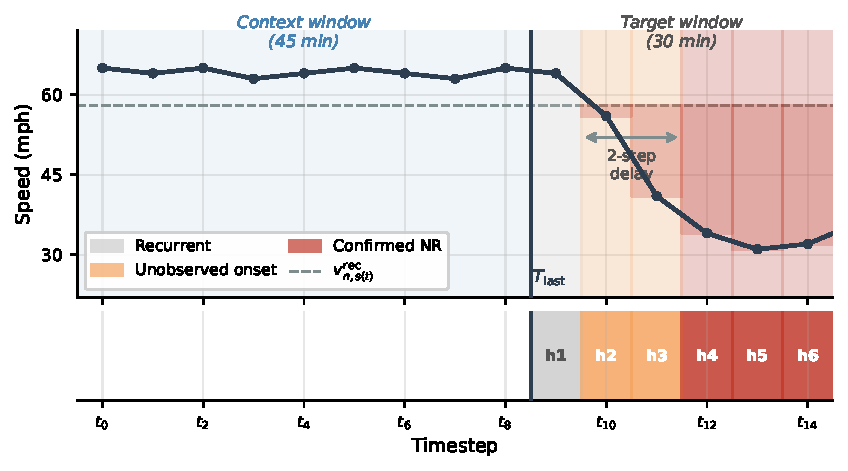
\includegraphics[width=\linewidth]{figures/regime_diagram.pdf}
  \caption{Illustration of the three evaluation regimes on a representative
           NR episode (TSMO, stylized speed trace).
           The context window (9 steps, 45~min) ends at $T_{\mathrm{last}}$
           (vertical line).
           Target steps h1--h6 are color-coded by regime: gray (recurrent),
           orange (unobserved onset), red (confirmed NR).
           The 2-step confirmation delay (10~min) at onset creates the
           unobserved onset regime; during these steps the model has no
           NR signal in context.
           All regime classification is per (prediction step, link).}
  \label{fig:regime_diagram}
\end{figure}

\subsection{Evaluation metrics}

For each regime $r \in \{\text{recurrent, onset, confirmed}\}$,
let $\Omega_r = \{(m, h, n) : r_{h,n}^{(m)} = r\}$ denote the set of
\textit{(sample, horizon, link)} triples belonging to that regime in the
test set.
We report the regime-stratified MAE, RMSE, and MAPE:
\begin{align}
  \text{MAE}_{r}    &= \frac{1}{|\Omega_r|}
    \sum_{(m,h,n) \in \Omega_r} \left|\hat{v}^{(m)}_{h,n} - v^{(m)}_{h,n}\right|,
    \label{eq:mae} \\
  \text{RMSE}_{r}   &= \sqrt{\frac{1}{|\Omega_r|}
    \sum_{(m,h,n) \in \Omega_r} \left(\hat{v}^{(m)}_{h,n} - v^{(m)}_{h,n}\right)^2},
    \label{eq:rmse} \\
  \text{MAPE}_{r}   &= \frac{100}{|\Omega_r|}
    \sum_{(m,h,n) \in \Omega_r}
    \frac{\left|\hat{v}^{(m)}_{h,n} - v^{(m)}_{h,n}\right|}
         {\left|v^{(m)}_{h,n}\right|},
    \label{eq:mape}
\end{align}
where $v^{(m)}_{h,n}$ and $\hat{v}^{(m)}_{h,n}$ are the true and
predicted speeds in original~mph units.
All three metrics are computed per-horizon ($h = 1,\dots,6$, i.e.\
5--30~min) and averaged across horizons.
The regime-stratified MAE is the primary reported metric.

% ══════════════════════════════════════════════════════════════
\section{Experimental Setup}
\label{sec:setup}
% ══════════════════════════════════════════════════════════════

\subsection{Study networks and data}
\label{sec:networks}

All experiments use 5-minute link-level probe vehicle speed data
derived from INRIX commercial GPS trajectories aggregated to Traffic
Message Channel~(TMC) segments, accessed via the Regional Integrated
Transportation Information System~(RITIS).
The same networks and preprocessing pipeline are used
in~\citet{bae2026labeling}, \citet{bae2026onset}, and~\citet{bae2026spatial}.
Figure~\ref{fig:networks} shows the spatial layout of both networks.

\begin{figure}[htbp]
  \centering
  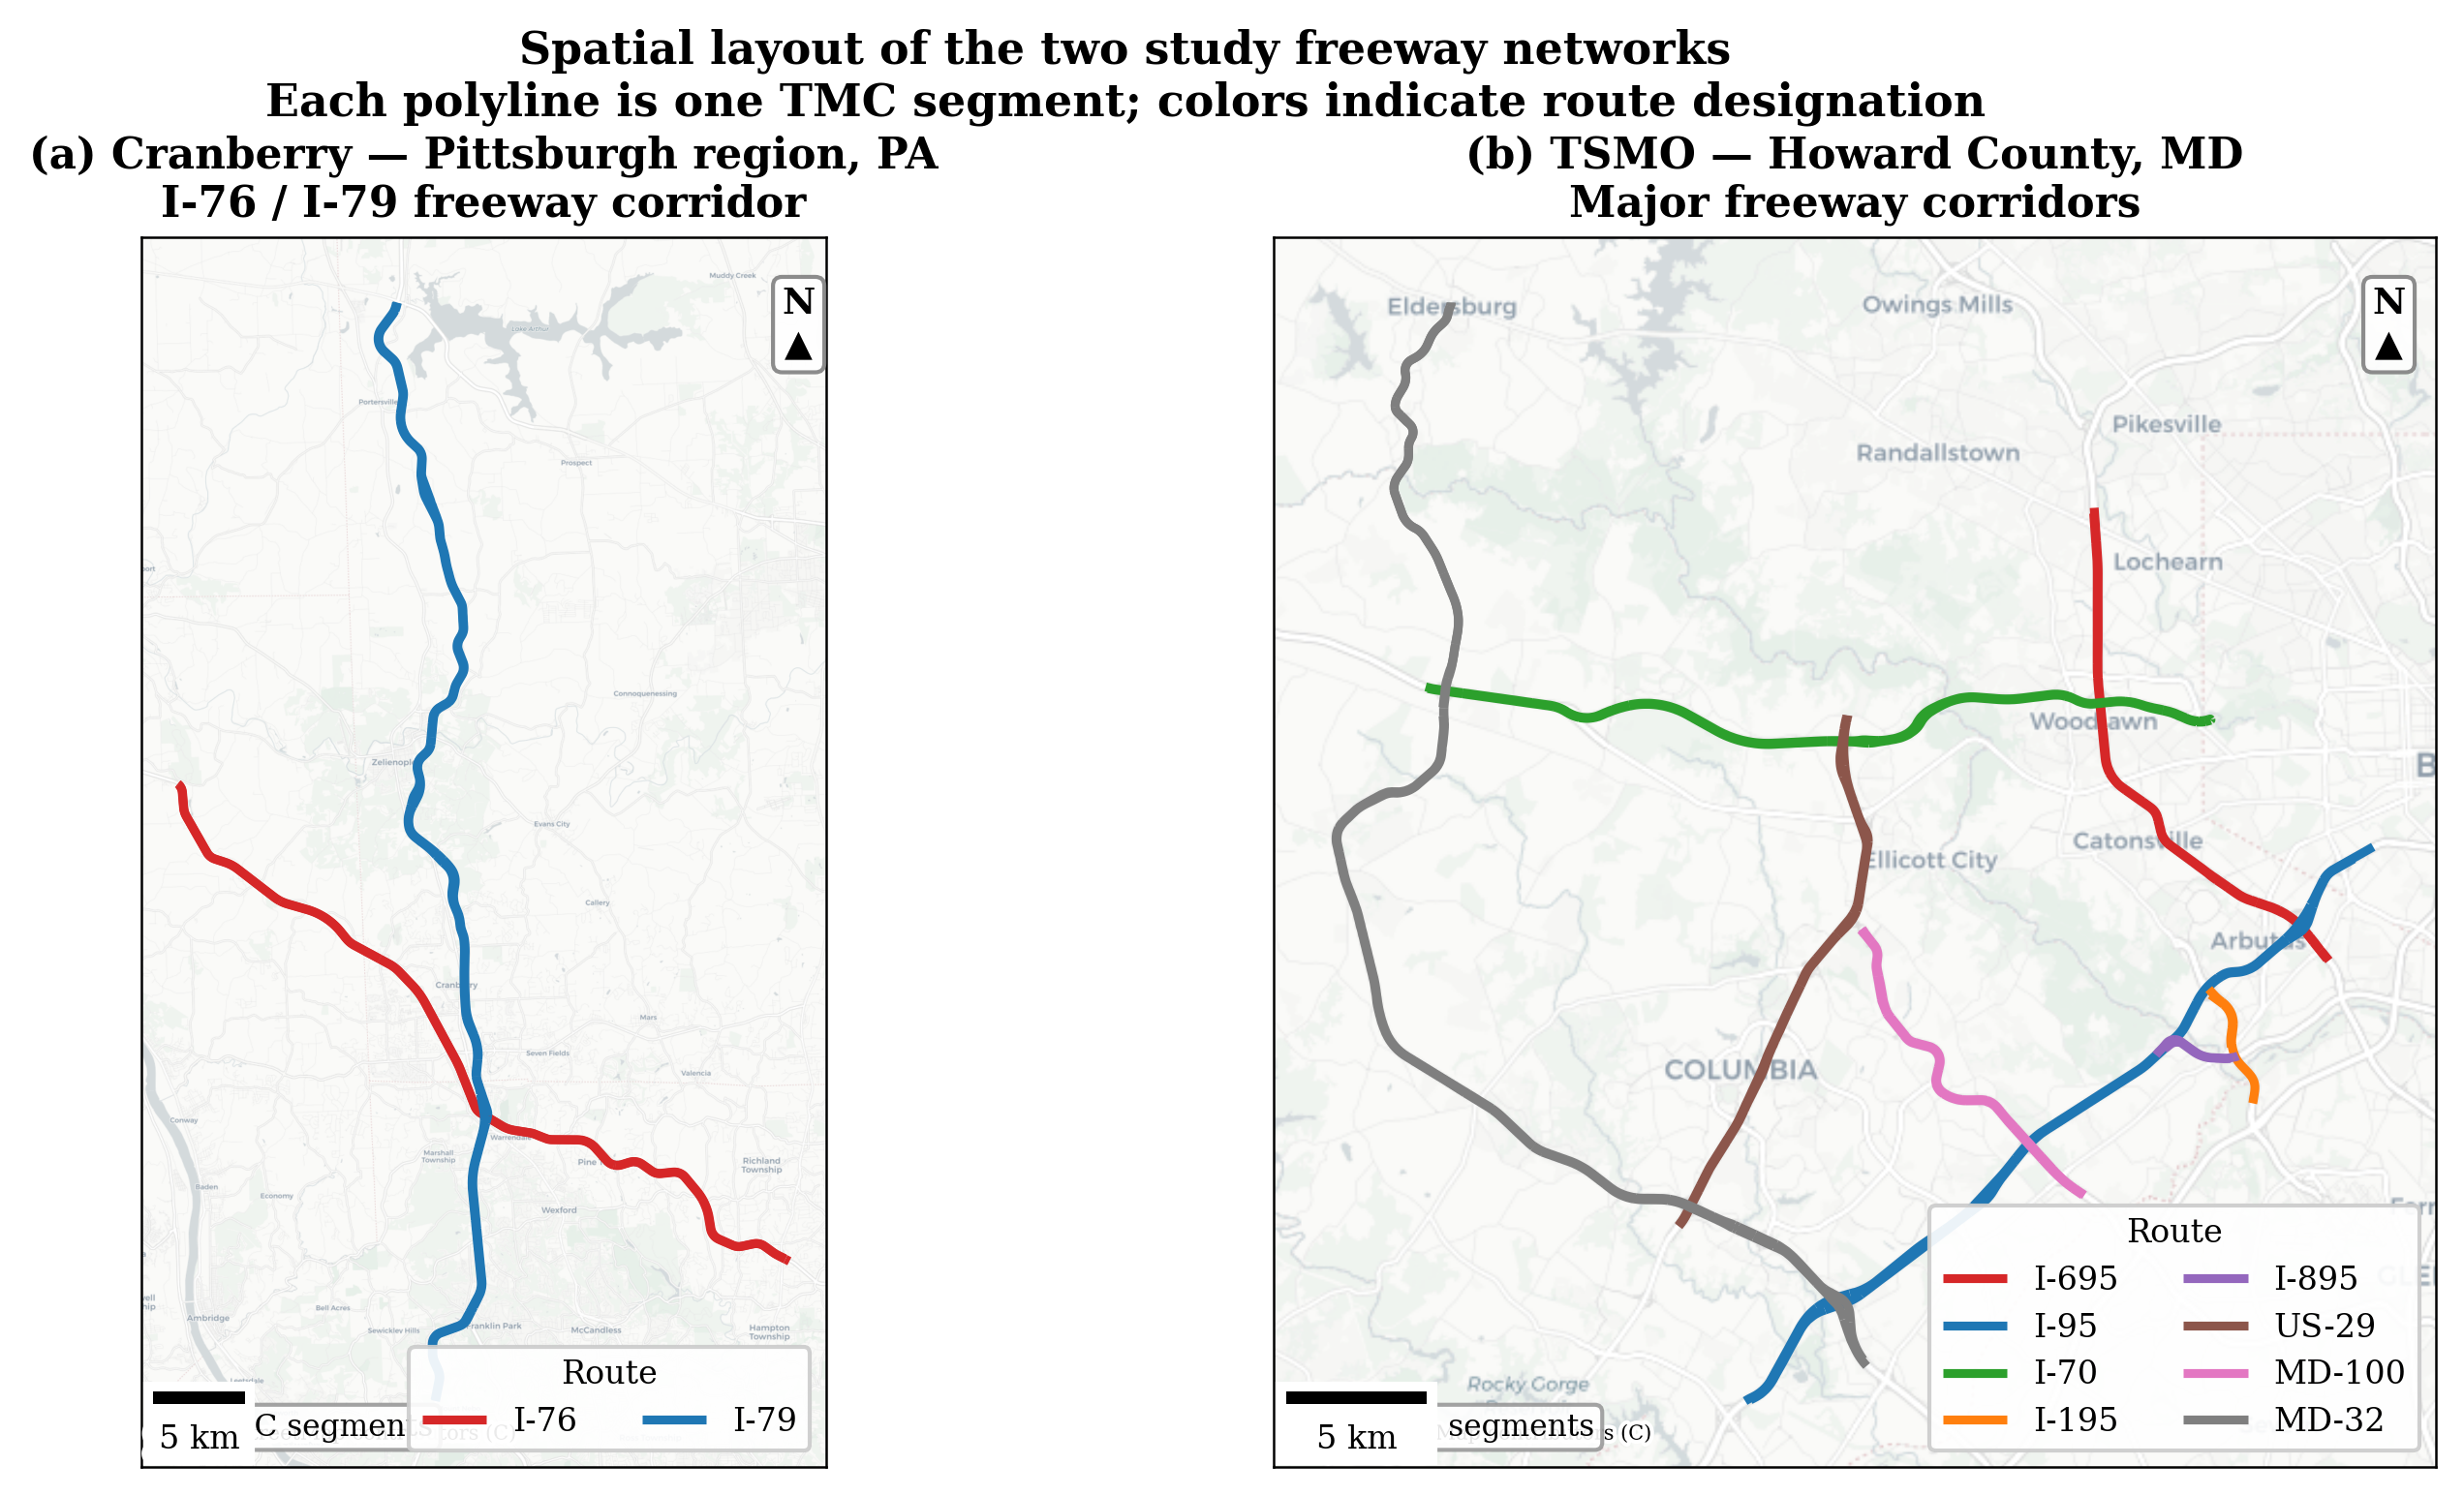
\includegraphics[width=\linewidth]{figures/networks.pdf}
  \caption{Spatial layout of the two study freeway networks.
           Each polyline is one TMC link; colors indicate route designation.
           (a)~Cranberry Township, PA: the I-76/I-79 freeway corridor
           ($N{=}78$ links, February 2022--January 2024, NR rate 2.42\%).
           (b)~TSMO network, Howard County, MD: eight major freeway
           corridors ($N{=}228$ links, February 2022--February 2023,
           NR rate 3.97\%).
           Source: INRIX probe vehicle data accessed via RITIS;
           network geometry from~\citet{bae2026labeling}.}
  \label{fig:networks}
\end{figure}

\paragraph{TSMO (Howard County, Maryland).}
The Transportation Systems Management and Operations~(TSMO) network
covers eight major freeway corridors in Howard County, Maryland:
I-695 (Baltimore Beltway), I-95 (Capital Beltway spur), I-70,
I-195, I-895, US-29, MD-100, and MD-32.
Segments are filtered to those with estimated free-flow speed above
50~mph, yielding $N = 228$ TMC links with a median segment length
of approximately 0.8~miles.
The observation period spans one full calendar year
($T = 48{,}360$ five-minute intervals, February 2022--February 2023).
The overall NR rate is 3.97\% of link-timesteps, rising to 5.12\%
in the validation split and falling to 3.01\% in the test split,
reflecting seasonal variation in incident activity.
Howard County is a heavily traveled suburban corridor connecting
Baltimore and Washington, DC, with high incident exposure on its
interchange-dense beltway and radial freeway segments.

\paragraph{Cranberry (Pittsburgh, Pennsylvania).}
The Cranberry network covers I-76 (Pennsylvania Turnpike) and I-79
near Cranberry Township, Butler County, a rapidly developing
exurban corridor north of Pittsburgh with significant incident
exposure from both high truck volumes (I-76) and commuter traffic (I-79).
The network comprises $N = 78$ TMC links observed over two full
years ($T = 97{,}092$ five-minute intervals,
February 2022--January 2024), providing a substantially larger
sample for cross-network replication.
The overall NR rate is 2.42\%, lower than TSMO, consistent with the
less complex interchange geometry and lower overall volume levels.

\paragraph{Temporal split.}
Both networks use a chronological 70/15/15 train/validation/test split
applied to the full time series without shuffling, preserving the
natural temporal ordering required for causal evaluation.
Sliding windows are session-aware: they never span overnight gaps
(after 20:55) or weekend/holiday operating boundaries,
so every window captures a contiguous operating period.
This yields 31,304 / 6,708 / 6,708 training/validation/test windows
for TSMO and 62,840 / 13,458 / 13,458 for Cranberry.

\paragraph{Speed data and NR labels.}
Speed data is the 5-minute average across all probe vehicles on each
TMC segment, sourced from INRIX via RITIS.
NR labels are produced by the ensemble detection framework
of~\citet{bae2026labeling}, which combines three interpretable
detectors (speed deviation, temporal gradient, upstream slowdown
contrast) with a 15-minute persistence filter.
The recurrent lower-bound reference speed $v^{\mathrm{rec}}_{n,s(t)}$
is estimated from the time-of-week distribution of the training set.

\paragraph{Weather and ancillary data.}
Weather features are derived from NOAA Integrated Surface Database
station data: 18 variables for TSMO (from 3 nearby stations) and
12 for Cranberry (from 2 stations), including temperature,
precipitation intensity, snowfall, wind speed, visibility, and
sky cover.
Crowd-sourced incident indicators are derived from Waze event
reports, spatially joined to TMC segments within a 0.5-mile
buffer and temporally matched to 5-minute intervals.
These ancillary features are used only in the feature configuration
ablation (Section~\ref{sec:results_features}); the core benchmark
uses speed only.

\subsection{Models}
\label{sec:models}

We evaluate 17 models spanning four families:

\paragraph{Statistical baselines (4).}
\textit{Last observation} (LO) persists the most recent observed speed.
\textit{Historical average} (HA) uses the same day-of-week and
time-of-day median from the training set.
\textit{Linear AR} fits a global Ridge regression on lagged speed,
time features, and link one-hot encodings.
\textit{XGBoost}~\citep{chen2016xgboost} is a global gradient-boosted
tree model with direct multi-step prediction.

\paragraph{Per-link deep learning (2).}
\textit{LSTM}~\citep{hochreiter1997lstm}: a two-layer Seq2Seq LSTM
encoder-decoder with shared weights across links.
\textit{Transformer}~\citep{vaswani2017attention}: a Seq2Seq Transformer
encoder-decoder with shared weights across links.

\paragraph{Spatial-temporal graph networks (11).}
We implement eleven models from the LargeST framework~\citep{liu2024largest}
via a unified adapter (\texttt{LargeSTRunner}) that standardizes
input and output formats:
HL, LSTM-ST, DCRNN~\citep{li2018dcrnn},
AGCRN~\citep{bai2020adaptive}, STGCN~\citep{yu2018stgcn},
Graph WaveNet (GWNet)~\citep{wu2019gwnet},
ASTGCN~\citep{guo2021astgcn}, STTN, STGODE~\citep{fang2021stgode},
DGCRN~\citep{li2023dgcrn}, D2STGNN~\citep{liu2023d2stgnn}.
All spatial models operate on the full graph with shared weights.

\paragraph{Training.}
All deep learning models are trained with Adam~\citep{kingma2015adam} ($\eta = 10^{-3}$,
weight decay $10^{-4}$), gradient clipping (norm~5), and early
stopping (patience~15 on validation MAE).
Statistical baselines require no training. ML baselines are trained
on the full training set.
Maximum 100 epochs; batch size 64.

\subsection{Feature configurations}
\label{sec:feature_configs}

\begin{table}[h]
\centering
\caption{Input feature configurations.
         $W$ = number of weather features (18 for TSMO, 12 for Cranberry).
         Time = time-of-day and day-of-week encodings.}
\label{tab:feature_configs}
\small
\begin{tabular}{lll}
\toprule
Configuration ID & Input channels & $C$ \\
\midrule
\texttt{speed}                       & Speed & 1 \\
\texttt{speed\_time}                 & Speed + Time & 3 \\
\texttt{speed\_incidents}            & Speed + Incidents & 2 \\
\texttt{speed\_nr}                   & Speed + Causal NR label & 2 \\
\texttt{speed\_weather}              & Speed + Weather & $1{+}W$ \\
\texttt{speed\_time\_incidents}      & Speed + Time + Incidents & 4 \\
\texttt{speed\_time\_nr}             & Speed + Time + Causal NR & 4 \\
\texttt{speed\_weather\_incidents}   & Speed + Weather + Incidents & $1{+}W{+}1$ \\
\texttt{speed\_time\_weather}        & Speed + Time + Weather & $3{+}W$ \\
\texttt{speed\_time\_weather\_incidents} & All features & $3{+}W{+}1$ \\
\bottomrule
\end{tabular}
\end{table}

The causal NR label channel (used in \texttt{speed\_nr} and
\texttt{speed\_time\_nr}) is constructed as
$y^{\mathrm{causal}}_{t,n}(T_{\mathrm{last}})$ from
Eq.~\eqref{eq:causal}: the label is set to~1 only if the NR episode
was confirmed by the end of the context window.
This preserves causal validity: no future information leaks into the
input.

\subsection{Training strategies}
\label{sec:strategies}

Four training objectives are evaluated (Section~\ref{sec:results_strategies}):

\paragraph{Standard.}
MSE loss over all target \textit{(step, link)} pairs, uniform weighting.

\paragraph{Weighted loss.}
MSE with per-\textit{(step, link)} upweighting of confirmed NR steps:
$w_{t,n} = 1 + (\lambda - 1)\causalfixed_{t,n}$,
where $\lambda$ is tuned on the validation NR~MAE.

\paragraph{NR fine-tuning.}
Two-phase training: (1)~standard MSE on all data for the first half
of the epoch budget; (2)~standard MSE on NR-containing windows only,
at reduced learning rate $\eta' = \mu \cdot \eta$, where $\mu$ is
tuned on validation NR~MAE.

\paragraph{Multi-objective.}
Speed MSE plus an auxiliary binary cross-entropy loss on the
confirmed NR label via a lightweight prediction head:
\begin{equation} \mathcal{L} = \mathcal{L}_{\text{speed}} + \gamma \mathcal{L}_{\text{NR}}. \label{eq:multi_obj} \end{equation}

Hyperparameters $\lambda$, $\mu$, and $\gamma$ are selected by grid
search on the TSMO validation NR~MAE and applied unchanged to Cranberry.

\subsection{Exclusions}
\label{sec:exclusions}

A small number of configurations could not be completed due to
numerical instability.
ASTGCN exhibits attention softmax overflow in fp32 for the
\texttt{multi\_objective} strategy on both networks and for
\texttt{nr\_finetune} on TSMO; these configurations are excluded.
D2STGNN produces non-finite loss on TSMO across all five
re-initialization attempts for every non-standard strategy, and its
saved results for those configurations are invalid.
All exclusions are documented in Appendix~\ref{app:exclusions}
and involve only 2 of 13 deep-learning models for TSMO non-standard
strategies; they do not affect any of the paper's primary conclusions.

% ══════════════════════════════════════════════════════════════
\section{Core Benchmark Results}
\label{sec:results_core}
% ══════════════════════════════════════════════════════════════

Tables~\ref{tab:phase1_tsmo} and~\ref{tab:phase1_cranberry} report the
core benchmark: all 17 models on the \texttt{speed}/\texttt{standard}
configuration on TSMO and Cranberry respectively.
Each row reports MAE (mph) for the full test set (Overall), the
recurrent regime, the unobserved onset regime, and the confirmed NR
regime, all averaged across the six forecast horizons (h1--h6,
5--30~min).
Models are grouped by family and sorted by confirmed NR MAE within each
family. The best confirmed NR MAE per family is shown in bold.

\begin{table}[htbp]
\centering
\caption{Phase~1 benchmark results on TSMO ($N{=}228$, 1~year),
         \texttt{speed}/\texttt{standard} configuration.
         All values are MAE in mph averaged over the six forecast
         horizons (h1--h6) unless otherwise noted.
         Columns h1--h6 show per-horizon NR MAE (combined onset and
         confirmed NR) at 5, 10, 15, 20, 25, and 30~min respectively.
         Bold: best confirmed NR MAE per family.
         NR rate in test set: 3.01\%.
         The section title uses 2--5$\times$ as a round bound that
         encompasses D2STGNN; the precise within-model range is 2.5--4.2$\times$
         excluding D2STGNN.
         $\dagger$~See Section~\ref{sec:finding3}.}
\label{tab:phase1_tsmo}
\small
\resizebox{\textwidth}{!}{%
\begin{tabular}{ll r r r r | r r r r r r}
\toprule
 & & \multicolumn{4}{c|}{Regime MAE (avg)} & \multicolumn{6}{c}{NR MAE by horizon (mph)} \\
\cmidrule(lr){3-6}\cmidrule(lr){7-12}
Family & Model & Overall & Recurrent & Onset & Conf.\ NR & h1 & h2 & h3 & h4 & h5 & h6 \\
\midrule
\multirow{4}{*}{Statistical / ML}
 & Last Obs.        & 4.852 & 4.646 & 14.383 &  9.577 &  6.168 &  8.867 & 11.113 & 12.513 & 13.514 & 14.215 \\
 & Hist.\ Avg.      & 4.878 & 4.590 & 13.568 & 13.558 & 13.580 & 13.573 & 13.567 & 13.557 & 13.548 & 13.542 \\
 & Linear AR        & 4.071 & 3.807 & 14.642 & 10.856 &  8.572 & 10.604 & 12.028 & 12.981 & 13.708 & 14.278 \\
 & \textbf{XGBoost} & 3.944 & 3.673 & 15.308 & \textbf{10.650} & 7.482 & 10.123 & 12.225 & 13.513 & 14.329 & 14.883 \\
\midrule
\multirow{2}{*}{Per-link DL}
 & LSTM             & 3.897 & 3.671 & 14.224 &  9.094 &  6.570 &  8.870 & 10.667 & 11.880 & 12.739 & 13.372 \\
 & \textbf{Transformer} & 3.872 & 3.644 & 14.466 & \textbf{9.081} &  6.538 &  8.890 & 10.714 & 11.972 & 12.860 & 13.519 \\
\midrule
\multirow{11}{*}{Spatial-temporal}
 & HL               & 4.852 & 4.646 & 14.383 &  9.577 &  6.168 &  8.867 & 11.113 & 12.513 & 13.514 & 14.215 \\
 & \textbf{DGCRN}   & 3.653 & 3.482 & 12.149 & \textbf{7.341} & 5.444 &  7.221 &  8.704 &  9.800 & 10.601 & 11.209 \\
 & GWNet            & 3.702 & 3.526 & 12.394 &  7.484 &  5.306 &  7.304 &  8.874 & 10.059 & 10.923 & 11.560 \\
 & STTN             & 3.680 & 3.501 & 12.377 &  7.602 &  5.281 &  7.356 &  8.974 & 10.168 & 11.037 & 11.670 \\
 & STGCN            & 3.715 & 3.532 & 12.515 &  7.772 &  5.786 &  7.566 &  9.090 & 10.229 & 11.071 & 11.702 \\
 & AGCRN            & 3.752 & 3.550 & 13.177 &  8.332 &  6.108 &  8.274 &  9.874 & 10.927 & 11.641 & 12.171 \\
 & DCRNN            & 3.813 & 3.614 & 13.295 &  8.247 &  5.936 &  8.016 &  9.664 & 10.898 & 11.826 & 12.523 \\
 & STGODE           & 3.794 & 3.589 & 13.555 &  8.355 &  5.754 &  7.986 &  9.791 & 11.168 & 12.167 & 12.925 \\
 & LSTM-ST          & 3.884 & 3.665 & 14.049 &  8.885 &  6.415 &  8.717 & 10.485 & 11.663 & 12.506 & 13.123 \\
 & ASTGCN           & 3.959 & 3.709 & 13.855 & 10.425 &  8.920 & 10.366 & 11.444 & 12.164 & 12.797 & 13.231 \\
 & D2STGNN$^\dagger$& 5.249 & 4.834 & 15.740 & 18.660 & 17.443 & 17.654 & 18.044 & 17.350 & 17.890 & 18.153 \\
\midrule
\multicolumn{2}{l}{\textit{Range (excl.\ D2STGNN)}} & 3.65--4.88 & 3.48--4.65 & 12.1--15.3 & 7.3--13.6 & 5.3--13.6 & 7.2--13.6 & 8.7--13.6 & 9.8--13.6 & 10.6--14.3 & 11.2--14.9 \\
\bottomrule
\end{tabular}}
\end{table}

\begin{table}[htbp]
\centering
\caption{Phase~1 benchmark results on Cranberry ($N{=}78$, 2~years),
         \texttt{speed}/\texttt{standard} configuration.
         Column definitions identical to Table~\ref{tab:phase1_tsmo}.
         NR rate in test set: 2.31\%.
         $\dagger$~See Section~\ref{sec:finding3}.}
\label{tab:phase1_cranberry}
\small
\resizebox{\textwidth}{!}{%
\begin{tabular}{ll r r r r | r r r r r r}
\toprule
 & & \multicolumn{4}{c|}{Regime MAE (avg)} & \multicolumn{6}{c}{NR MAE by horizon (mph)} \\
\cmidrule(lr){3-6}\cmidrule(lr){7-12}
Family & Model & Overall & Recurrent & Onset & Conf.\ NR & h1 & h2 & h3 & h4 & h5 & h6 \\
\midrule
\multirow{4}{*}{Statistical / ML}
 & Last Obs.        & 4.479 & 4.371 & 12.151 &  7.735 &  6.826 &  8.155 &  9.081 &  9.499 &  9.747 &  9.941 \\
 & Hist.\ Avg.      & 3.812 & 3.612 & 13.129 & 11.567 & 12.030 & 12.003 & 11.973 & 11.950 & 11.937 & 11.916 \\
 & Linear AR        & 3.433 & 3.322 & 11.656 &  6.688 &  6.788 &  7.589 &  8.023 &  8.282 &  8.474 &  8.649 \\
 & \textbf{XGBoost} & 3.380 & 3.274 & 11.616 & \textbf{6.328} &  6.354 &  7.221 &  7.734 &  8.059 &  8.300 &  8.476 \\
\midrule
\multirow{2}{*}{Per-link DL}
 & LSTM             & 3.384 & 3.280 & 11.597 &  6.240 &  6.205 &  7.094 &  7.643 &  8.008 &  8.267 &  8.508 \\
 & \textbf{Transformer} & 3.377 & 3.274 & 11.674 & \textbf{6.164} & 6.266 & 7.074 & 7.588 & 7.936 & 8.202 & 8.440 \\
\midrule
\multirow{11}{*}{Spatial-temporal}
 & HL               & 4.479 & 4.371 & 12.151 &  7.735 &  6.826 &  8.155 &  9.081 &  9.499 &  9.747 &  9.941 \\
 & \textbf{DGCRN}   & 3.247 & 3.153 & 11.109 & \textbf{5.668} & 5.646 &  6.549 &  7.060 &  7.437 &  7.742 &  7.987 \\
 & GWNet            & 3.221 & 3.126 & 11.215 &  5.671 &  5.613 &  6.543 &  7.095 &  7.492 &  7.806 &  8.049 \\
 & STTN             & 3.254 & 3.157 & 11.258 &  5.814 &  5.673 &  6.689 &  7.220 &  7.593 &  7.937 &  8.191 \\
 & STGCN            & 3.280 & 3.182 & 11.167 &  5.926 &  5.916 &  6.756 &  7.263 &  7.618 &  7.921 &  8.185 \\
 & AGCRN            & 3.276 & 3.177 & 11.395 &  5.908 &  5.955 &  6.816 &  7.331 &  7.682 &  7.952 &  8.194 \\
 & DCRNN            & 3.267 & 3.165 & 11.225 &  6.106 &  5.821 &  6.776 &  7.355 &  7.820 &  8.211 &  8.574 \\
 & STGODE           & 3.352 & 3.252 & 11.546 &  5.983 &  6.007 &  6.859 &  7.405 &  7.792 &  8.090 &  8.345 \\
 & LSTM-ST          & 3.383 & 3.281 & 11.602 &  6.169 &  6.221 &  7.061 &  7.582 &  7.931 &  8.187 &  8.435 \\
 & ASTGCN           & 3.452 & 3.328 & 11.799 &  7.389 &  7.947 &  8.271 &  8.493 &  8.668 &  8.808 &  8.958 \\
 & D2STGNN$^\dagger$& 3.793 & 3.587 & 13.352 & 11.792 & 12.055 & 12.142 & 12.358 & 11.968 & 12.221 & 12.415 \\
\midrule
\multicolumn{2}{l}{\textit{Range (excl.\ D2STGNN)}} & 3.22--4.48 & 3.13--4.37 & 11.1--13.1 & 5.7--7.7 & 5.6--7.9 & 6.5--8.2 & 7.1--9.1 & 7.4--9.5 & 7.7--9.7 & 8.0--9.9 \\
\bottomrule
\end{tabular}}
\end{table}

\subsection{NR MAE is 2--5$\times$ higher than recurrent MAE}
\label{sec:finding1}

Across all models and both networks, NR~MAE substantially exceeds
recurrent~MAE.
On TSMO, recurrent MAE spans 3.48--4.65~mph across all non-trivial
models, while the combined NR~MAE spans 8.83--17.76~mph,
a ratio of 2.5--4.2$\times$ when excluding the D2STGNN outlier.
The median NR-to-recurrent MAE ratio across all non-trivial TSMO models
is approximately 2.8$\times$.
On Cranberry the ratio is somewhat smaller: recurrent 3.13--4.37~mph,
NR 7.07--11.97~mph (ratio 2.0--3.3$\times$, median $\approx 2.4\times$),
consistent with Cranberry's lower NR rate (2.31\% versus 3.01\% on TSMO).
The combined NR~MAE metric averages over onset and confirmed NR samples
and is not shown as a separate column in
Tables~\ref{tab:phase1_tsmo}--\ref{tab:phase1_cranberry},
which report onset and confirmed NR MAE separately.

This gap is not model-specific: it holds for simple baselines (historical
average ratio $2.95\times$ on TSMO), linear models (linear AR,
$3.16\times$), per-link neural networks (LSTM $2.91\times$, Transformer
$2.95\times$), and graph-based spatiotemporal architectures
($2.54\times$ for DGCRN, the best spatial model).
No architecture closes the NR gap to below $2\times$ on either network.

\subsection{Onset is the dominant failure mode}
\label{sec:finding2}

The causal observability framework reveals that NR error is not
uniform: onset MAE is consistently and substantially higher than
confirmed NR~MAE across all models and both networks.

On TSMO, onset MAE for the best spatial models (DGCRN, GWNet, STTN)
ranges 12.1--12.4~mph, while confirmed NR MAE for the same models
is 7.3--7.6~mph, meaning onset MAE is 60--70\% higher than confirmed
NR MAE within the NR regime.
The same pattern holds on Cranberry (onset 11.1--11.3~mph,
confirmed 5.7--5.9~mph for the best spatial models),
where the onset-to-confirmed ratio is approximately $1.9\times$.

This finding has a direct interpretation through the causal
observability framework (Section~\ref{sec:causal}).
In the confirmed NR regime, the model observes a confirmed NR
signal in its context window; it knows a disturbance is active
and must predict its continuation or recovery.
In the unobserved onset regime, the model is informationally blind:
the disturbance has begun but has not yet been confirmed,
and the context window contains no NR signal to exploit.
The 60--70\% onset penalty quantifies the cost of this informational
blindness and cannot be reduced by improving model capacity alone,
since even a perfect model has no access to the unconfirmed onset
signal.

Strikingly, even the historical average model has competitive onset
MAE on TSMO (13.57~mph), within 12\% of the best spatial models
(12.15~mph for DGCRN).
Since the historical average makes no use of recent observations,
this suggests that a substantial fraction of onset difficulty is
inherent to the informational structure of the problem rather than
to model quality.

\subsection{Model rankings shift under NR evaluation}
\label{sec:finding3}

While aggregate MAE rankings and NR MAE rankings are broadly
correlated (the best aggregate models also tend to be the best
NR models), meaningful differences emerge that have
operational implications.

On TSMO, the historical average (overall: 4.878~mph) ranks among the
weakest models on aggregate MAE, far behind LSTM~(3.897~mph)
and Transformer~(3.872~mph).
On onset MAE, however, the historical average (13.57~mph) outperforms
both LSTM~(14.22~mph) and Transformer~(14.47~mph), reversing the
aggregate ordering.
The reversal has a structural explanation: during unobserved onset,
the speed has begun degrading but no NR signal is confirmed; per-link
networks that extrapolate recent dynamics may amplify the nascent
degradation, whereas the historical average's inertia toward normal
conditions becomes advantageous.

The spatial models present a more nuanced picture.
On both networks, DGCRN, GWNet, and STTN achieve the lowest NR~MAE
among spatial models, consistent with their aggregate rankings.
However, ASTGCN, which is competitive in aggregate MAE (3.959~mph
on TSMO), has substantially higher NR MAE (onset: 13.86~mph) than
simpler spatial models with similar aggregate performance.
We speculate that ASTGCN's known numerical sensitivity
(Section~\ref{sec:exclusions}) may contribute to this pattern,
though the relationship is not established.

One anomaly requires specific discussion.
\emph{D2STGNN on TSMO} produces consistently poor NR performance
(combined NR~MAE: 17.76~mph, onset: 15.74~mph, confirmed NR: 18.66~mph)
across all ten feature configurations, placing it far below all
other models including simple baselines.
In contrast, D2STGNN on Cranberry achieves competitive overall
performance (3.793~mph) but still elevated NR~MAE (12.19~mph).
The TSMO-specific failure is consistent with D2STGNN's instability
on that network (Appendix~\ref{app:exclusions}) and may reflect
interactions between its internal time-embedding architecture and
the longer, more variable TSMO episodes.
D2STGNN is retained in the tables for completeness but excluded
from aggregate range statistics.

\subsection{Cross-network replication}
\label{sec:replication}

The three core findings replicate across both networks:
(1)~NR MAE substantially exceeds recurrent MAE on Cranberry
(median $2.4\times$) as on TSMO ($2.8\times$);
(2)~onset MAE substantially exceeds confirmed NR MAE on both
networks (TSMO $\approx 1.7\times$, Cranberry $\approx 1.9\times$);
(3)~the best NR models on Cranberry are DGCRN and GWNet
(confirmed NR MAE $\approx$5.67~mph), the same architectures that
dominate on TSMO.

The absolute NR~MAE values are lower on Cranberry than TSMO for
comparable models, consistent with Cranberry's lower NR rate.
The ranking structure within the spatial family is stable:
DGCRN, GWNet, and STTN lead on both networks.

An important pattern emerges across both networks:
for the onset regime specifically, the gap between the best spatial
models and simple baselines is modest relative to the recurrent regime.
On TSMO, DGCRN onset MAE (12.15~mph) is within 12\% of the
historical average onset MAE (13.57~mph), whereas the aggregate
gap between the two is 33\%.
This suggests that spatial context provides meaningful but limited
benefit for onset prediction, consistent with the binary onset
prediction findings of~\citet{bae2026onset}, who find that graph
convolution improves onset F1 by approximately $2\times$ over
local models but leaves all models far below operational thresholds.

% ══════════════════════════════════════════════════════════════
\section{Feature Configuration Results}
\label{sec:results_features}
% ══════════════════════════════════════════════════════════════

Phase~2 evaluates whether richer input features improve NR performance.
We report NR~MAE for each of the ten feature configurations
(Table~\ref{tab:feature_configs}) under the standard training objective
for all 17 models.

\subsection{Effect of Feature Enrichment on NR MAE}

Table~\ref{tab:phase2_summary} summarizes the median NR~MAE across
all non-excluded models for each feature configuration,
relative to the \texttt{speed}-only baseline.

\begin{table}[htbp]
\centering
\caption{Phase~2 results: median NR~MAE (mph) across all non-excluded
         models by feature configuration, \texttt{standard} strategy.
         Medians computed over 16 models per cell (13 for
         \texttt{speed\_nr} on TSMO, which uses the
         \texttt{speed\_nr\_causal} variant).
         $\Delta$ = reduction relative to \texttt{speed} baseline
         (positive = improvement; negative = degradation).
         Bold: best per network; ties broken by configuration simplicity.
         D2STGNN excluded from all medians.}
\label{tab:phase2_summary}
\small
\begin{tabular}{lrr rr}
\toprule
 & \multicolumn{2}{c}{TSMO} & \multicolumn{2}{c}{Cranberry} \\
\cmidrule(lr){2-3}\cmidrule(lr){4-5}
Feature config & NR MAE & $\Delta$ & NR MAE & $\Delta$ \\
\midrule
\texttt{speed}                       & 10.58 & (base) &  7.58 & (base) \\
\texttt{speed\_time}                 & 10.04 & +0.54  &  7.56 & +0.01  \\
\texttt{speed\_incidents}            & 10.66 & $-$0.08 & 7.55 & +0.02  \\
\texttt{speed\_nr}                   & 10.47 & +0.11  &  7.64 & $-$0.06 \\
\texttt{speed\_weather}              & 10.30 & +0.28  &  7.71 & $-$0.13 \\
\texttt{speed\_time\_incidents}      & 10.00 & +0.58  &  7.53 & +0.05  \\
\textbf{\texttt{speed\_time\_nr}}    & \textbf{9.93} & \textbf{+0.65} & 7.62 & $-$0.04 \\
\texttt{speed\_weather\_incidents}   & 10.14 & +0.44  &  7.62 & $-$0.04 \\
\texttt{speed\_time\_weather}        & 10.22 & +0.36  &  7.65 & $-$0.08 \\
\texttt{speed\_time\_weather\_incidents} & 10.12 & +0.47 & \textbf{7.53} & \textbf{+0.05} \\
\bottomrule
\end{tabular}
\end{table}

The central finding is that feature enrichment does not solve the
NR prediction problem.
On TSMO, the best configuration (\texttt{speed\_time\_nr}) reduces
median NR~MAE by 0.65~mph (6.2\% relative to the \texttt{speed}
baseline), a real but small improvement relative to the 2.8$\times$
NR-to-recurrent gap.
On Cranberry, no feature configuration improves NR~MAE by more than
0.05~mph (0.7\%), and several weather-containing configurations are
marginally \emph{worse} than the speed-only baseline.
Feature enrichment, in other words, works modestly on one network
and not at all on the other.

Three patterns emerge from the TSMO results.
First, temporal features (\texttt{time}: TOD and DOW encodings) are
consistently the most valuable single addition, reducing median
NR~MAE by 0.54~mph (+5.1\%).
Second, combining temporal features with either the causal NR label
or incident indicators provides the largest improvements
(\texttt{speed\_time\_nr}: +0.65~mph, +6.2\%;
\texttt{speed\_time\_incidents}: +0.58~mph, +5.5\%).
Third, weather features alone provide only modest benefit (+0.28~mph),
and incident features alone provide essentially none
($-$0.08~mph, slightly worse than baseline).

Crucially, the causal NR label improves NR~MAE only in the
\emph{confirmed NR regime} where an episode is active in the context
window; it cannot help in the unobserved onset regime by construction.
The absence of any meaningful Cranberry improvement suggests that the
TSMO benefit is partly network-specific: TSMO's higher NR rate (3.01\%
in test) provides more confirmed NR training signal for the additional
features to exploit.

The maximum feature benefit (6.2\% on TSMO) is small relative to the
2.8$\times$ NR-to-recurrent gap and is entirely absent on Cranberry.
Richer inputs partially close the confirmed NR portion of the gap
on TSMO but do not address the unobserved onset problem on either network.

\subsection{Model sensitivity to feature configuration}

Feature response varies by model family.
Statistical models (linear AR, historical average) produce identical results across
feature configurations in our implementation, because they read only the speed
channel regardless of the feature configuration ID.
Per-link neural networks (LSTM, Transformer) show moderate
sensitivity; individually, their NR~MAE improves by approximately
10--15\% from \texttt{speed} to \texttt{speed\_time\_weather\_incidents}
on TSMO (not directly shown in Table~\ref{tab:phase2_summary},
which reports medians across all model families).
Spatial models show heterogeneous responses: DGCRN accepts
only the speed channel regardless of feature configuration due to
residual connection constraints (see Appendix~\ref{app:architectures}),
while models such as AGCRN and GWNet show the largest
absolute improvements from temporal features.

% ══════════════════════════════════════════════════════════════
\section{Training Strategy Results}
\label{sec:results_strategies}
% ══════════════════════════════════════════════════════════════

Phase~3 evaluates whether NR-aware training objectives improve NR~MAE
beyond what the standard MSE objective achieves.
We compare four strategies (Section~\ref{sec:strategies}) on the
\texttt{speed} feature configuration for all 13 deep learning models.
Excluded configurations are listed in Appendix~\ref{app:exclusions}.

\subsection{NR-aware training does not meaningfully reduce NR MAE}

Table~\ref{tab:phase3_summary} summarizes the median NR~MAE by
strategy across all non-excluded DL models.

\begin{table}[htbp]
\centering
\caption{Phase~3 results: median NR~MAE (mph) by training strategy
         across all non-excluded DL models, \texttt{speed} feature config.
         $\Delta$ = reduction relative to \texttt{standard}
         (positive = improvement; negative = degradation).
         TSMO: $n{=}13$ models for standard/weighted\_loss,
         $n{=}12$ for nr\_finetune/multi\_objective (D2STGNN excluded).
         Cranberry: $n{=}13$ (standard/weighted\_loss/nr\_finetune), $n{=}12$ (multi\_objective).
         Bold: best per network; ties broken by configuration simplicity.}
\label{tab:phase3_summary}
\small
\begin{tabular}{lrr rr}
\toprule
 & \multicolumn{2}{c}{TSMO} & \multicolumn{2}{c}{Cranberry} \\
\cmidrule(lr){2-3}\cmidrule(lr){4-5}
Strategy & NR MAE & $\Delta$ & NR MAE & $\Delta$ \\
\midrule
\texttt{standard}                           & 9.97 & (base) & 7.50 & (base) \\
\texttt{weighted\_loss}                     & 9.99 & $-$0.02 & 7.48 & +0.01 \\
\textbf{\texttt{nr\_finetune}}              & \textbf{9.86} & \textbf{+0.10} & \textbf{7.43} & \textbf{+0.07} \\
\texttt{multi\_objective}                   & 9.89 & +0.07 & 7.49 & +0.01 \\
\bottomrule
\end{tabular}
\end{table}

NR-aware training strategies do not meaningfully improve NR MAE.
The median improvements across all non-excluded DL models are
sub-1\% on both networks: the best strategy (\texttt{nr\_finetune})
achieves 0.10~mph (1.0\%) on TSMO and 0.07~mph (0.9\%) on Cranberry.
Crucially, \texttt{weighted\_loss} is marginally \emph{worse} than
standard on TSMO ($-$0.02~mph), directly contradicting the intuition
that upweighting NR steps in the loss should improve NR performance.
This is consistent with the 3.01\% NR rate in the TSMO training set:
the NR signal is too sparse at the batch level to provide a reliable
upweighting gradient.
We caution that differences of this magnitude (less than 0.1~mph) are
well within the expected inter-run variance for these models and
should not be interpreted as reliable improvements; we report them
for completeness and transparency rather than as evidence of
strategy effectiveness.

\subsection{Strategy benefit is model-dependent and inconsistent}

The medians in Table~\ref{tab:phase3_summary} conceal substantial
heterogeneity across models.
For some models (DCRNN, GWNet on Cranberry), NR-aware training
provides improvements of 5--8\% in NR~MAE relative to standard.
For others (AGCRN, STGODE), the strategies provide negligible
improvement or are marginally worse.
No single strategy dominates across all models and both networks.

The \texttt{weighted\_loss} result on TSMO is particularly instructive:
despite explicitly upweighting NR steps in the loss, median NR~MAE
is marginally higher than standard (9.99 vs 9.97~mph).
This suggests that the 3.01\% NR rate in the training set is too
sparse to provide a reliable upweighting signal at the batch level.
\texttt{nr\_finetune}, which concentrates the NR signal in a
dedicated fine-tuning phase, achieves more consistent improvements.

\subsection{The onset gap is not reduced by training strategies}

Perhaps the most important finding from the strategy comparison is
that NR-aware training does not meaningfully reduce onset~MAE.
Improvements are concentrated in the confirmed NR regime
(where the model has a confirmed NR signal in context and
the upweighted or auxiliary loss provides a useful gradient signal),
while onset~MAE remains essentially unchanged across strategies.
This is structurally expected: during the unobserved onset regime,
no NR signal is present in the context window, so no loss function
that upweights NR context steps can provide gradient information
for onset prediction.

% ══════════════════════════════════════════════════════════════
\section{Discussion}
\label{sec:discussion}
% ══════════════════════════════════════════════════════════════

\subsection{The nature of the NR gap}

The central finding of this study is that the NR MAE gap is large,
consistent, and structurally resistant to both richer inputs and
NR-aware training.
The 2--5$\times$ gap between NR and recurrent MAE persists across 17
models spanning four families of increasing architectural complexity,
two independent networks, ten input configurations, and four training
strategies.
The best single feature configuration reduces NR MAE by 6.2\% on TSMO
and essentially nothing on Cranberry.
The best training strategy adds at most 1.0\% on TSMO, and
\texttt{weighted\_loss} is marginally counterproductive.
Taken together, all of the modeling interventions we tested close
at most 7\% of the NR gap on the more responsive network and
nothing on the less responsive one.

This is not primarily a capacity problem.
The gap does not narrow with model complexity:
even the historical average model achieves onset MAE within 12\% of
DGCRN (the best spatial architecture) on TSMO, and simple linear AR
is within 20\%.
The bottleneck is informational, not architectural.
The unobserved onset regime presents a fundamentally hard prediction
problem where the model has no confirmed signal of the unfolding
event and must rely on weak pre-episode speed signatures.

\subsection{Implications for benchmark design}

Aggregate MAE evaluations on standard benchmarks do not reveal this
failure mode.
Because NR episodes occupy only 2--5\% of test samples, a model
that performs twice as poorly during NR episodes but accurately
predicts routine conditions can appear nearly identical to a
robust model in aggregate evaluation.
The causal observability framework introduced in this paper provides
a principled decomposition that makes the failure visible.
Separating onset (informationally blind) from confirmed NR
(model has a confirmed signal) from recurrent (baseline)
allows researchers to identify where in the episode structure
errors are concentrated and to design targeted improvements.

We recommend that future traffic forecasting papers report
regime-stratified MAE as a standard companion to aggregate MAE,
particularly when NR robustness is claimed.
A model that achieves low aggregate MAE but fails to reduce onset MAE
below simple baselines provides no practical early-warning advantage.

\subsection{Implications for operational deployment}

The confirmed NR regime is more tractable than onset and can be
partially addressed by richer inputs and NR-aware training.
Models with confirmed NR context achieve MAE approximately 30--40\%
lower than models in the onset regime, and temporal features provide
an additional 5--10\% improvement.
This suggests that for operational systems where incident reports
or NR detection outputs can be incorporated as real-time features,
meaningful accuracy gains are achievable during the confirmed phase.

The onset regime, however, represents the period of greatest
operational value (5--15 minutes before the episode is confirmed~\citep{fhwa2025})
and the period of greatest model failure.
Closing the onset gap likely requires approaches beyond the modeling
choices tested here: hybrid physical models that can propagate
upstream signatures before threshold crossing, pre-trained
representations of rare speed patterns, or ensemble methods that
aggregate weak pre-onset signals.

% ══════════════════════════════════════════════════════════════
\section{Conclusion}
\label{sec:conclusion}
% ══════════════════════════════════════════════════════════════

We present one of the first large-scale empirical benchmarks of
traffic speed forecasting under nonrecurrent conditions using a
causally grounded, per-link, per-timestep evaluation framework.
The causal observability framework formalizes the confirmation delay
inherent in real-time NR detection and partitions the evaluation
into three informationally distinct regimes: recurrent, unobserved
onset, and confirmed NR.

Across 17 models, two freeway networks, ten feature configurations,
and four training strategies, we find:
\begin{itemize}
  \item NR MAE is 2.5--3.2$\times$ higher than recurrent MAE for the
        best spatial models on TSMO (DGCRN: 2.54$\times$), and
        2.0--3.3$\times$ on Cranberry; across all 17 model families the
        range is 2--5$\times$ (Tables~\ref{tab:phase1_tsmo}--\ref{tab:phase1_cranberry}),
        with no architecture closing the gap below $2\times$ on either network.
  \item Unobserved onset is the dominant failure mode: onset MAE
        exceeds confirmed NR MAE by 60--70\% for the best spatial
        models on TSMO and $\approx 2\times$ on Cranberry.
        The historical average model achieves onset MAE within 12\%
        of DGCRN on TSMO despite being 33\% worse in aggregate.
        This contrast illustrates the informational rather than
        architectural nature of the onset bottleneck.
  \item Model rankings shift under NR evaluation.
        The historical average outperforms LSTM and Transformer
        on onset MAE on TSMO despite ranking far below them in
        aggregate.
  \item Feature enrichment reduces median NR MAE by at most 6.2\%
        on TSMO (\texttt{speed\_time\_nr}) and less than 1\% on
        Cranberry; improvements are concentrated in the confirmed NR
        regime and absent in the onset regime.
  \item NR-aware training strategies reduce median NR~MAE by at most
        1.0\% (\texttt{nr\_finetune} on TSMO); \texttt{weighted\_loss}
        is marginally counterproductive on TSMO.
        No strategy reduces onset~MAE meaningfully.
\end{itemize}

All findings replicate across both networks.
These results call for regime-stratified evaluation as a standard
reporting practice in traffic forecasting, and motivate
future work on onset-specific architectures and pre-episode signal
detection.
Further improvement remains possible
for improvement: hybrid physics-based models that propagate upstream
signatures before threshold crossing, and representations pre-trained
on rare speed patterns, remain unexplored.

\section*{CRediT Authorship Contribution Statement}

\textbf{Andrew J.~Bae}: Conceptualization, Data Curation, Software,
Methodology, Formal Analysis, Writing -- Original Draft,
Writing -- Review \& Editing.

\section*{Data and Code Availability}

Speed data are derived from INRIX commercial probe vehicle
observations accessed via RITIS under a data-use agreement and
cannot be redistributed.
NR labels, network topology files, model implementations, and
evaluation code are publicly available at
\texttt{[repository URL to be added upon acceptance]}.

\section*{Generative AI Statement}

Generative AI tools assisted with language editing.
All analysis, interpretation, and conclusions are the authors' own.

\section*{Competing Interests}

The author declares no competing interests.

\section*{Funding}

This work was supported by Fujitsu Research of America, Safety21
(the USDOT University Transportation Center for Safety, Mobility,
and Accessibility), and the Department of Civil and Environmental
Engineering at Carnegie Mellon University.
The funders had no role in the design of this paper.

\section*{Acknowledgements}

The author thanks Prof.~Sean Qian (CMU) for project supervision
and Haocheng Duan for discussions on NR labeling methodology.

% ══════════════════════════════════════════════════════════════
%% Appendix
% ══════════════════════════════════════════════════════════════
\appendix

\section{Known Exclusions}
\label{app:exclusions}

Table~\ref{tab:exclusions} lists all configurations excluded from the
benchmark due to numerical instability.

\begin{table}[h]
\centering
\caption{Excluded configurations and reasons.
         All excluded models have valid standard-strategy results
         on both networks (included in Section~\ref{sec:results_core}).}
\label{tab:exclusions}
\small
\begin{tabular}{lllp{6.5cm}}
\toprule
Network & Model & Strategy & Reason \\
\midrule
TSMO      & ASTGCN  & \texttt{multi\_objective} & fp32 attention softmax overflow in training; 5 re-initialization attempts failed \\
TSMO      & ASTGCN  & \texttt{nr\_finetune}     & fp32 attention softmax overflow in training; 5 re-initialization attempts failed \\
Cranberry & ASTGCN  & \texttt{multi\_objective} & fp32 attention softmax overflow in training; 5 re-initialization attempts failed \\
TSMO      & D2STGNN & \texttt{weighted\_loss}   & NaN loss from initialization; 5 re-init attempts failed; untrained-model predictions saved \\
TSMO      & D2STGNN & \texttt{nr\_finetune}     & NaN loss from initialization; 5 re-init attempts failed; untrained-model predictions saved \\
TSMO      & D2STGNN & \texttt{multi\_objective} & NaN loss from initialization; 5 re-init attempts failed; untrained-model predictions saved \\
\bottomrule
\end{tabular}
\end{table}

ASTGCN's instability in fp32 is a known limitation of its attention
architecture (the model is already excluded from AMP training for this
reason).
D2STGNN's instability on TSMO is consistent with its anomalously
poor standard-strategy performance on the same network
(Section~\ref{sec:finding3}), and suggests a fundamental
compatibility issue between D2STGNN's internal architecture and
the TSMO graph at $N{=}228$.
GWNet, which previously also failed due to CUDA driver state
corruption, completed all three non-standard strategies on TSMO
after a clean session restart and is fully included.

The exclusions affect only the training strategy comparison
(Section~\ref{sec:results_strategies}) and involve 2 out of 13
deep learning models for TSMO non-standard strategies,
leaving 11 models fully covered on both networks for all strategies.

% ══════════════════════════════════════════════════════════════
\section{Compute Resources and Training Times}
\label{app:compute}
% ══════════════════════════════════════════════════════════════

\subsection{Hardware}

All deep learning experiments were conducted on a JupyterHub cluster
node with the following configuration:
\begin{itemize}
  \item \textbf{GPU:} NVIDIA A100~80GB PCIe, accessed via a
        3g.40gb MIG partition (40~GB dedicated GPU memory)
  \item \textbf{CPU:} 48 cores
  \item \textbf{RAM:} 128~GB
  \item \textbf{CUDA:} 13.0; PyTorch 2.x
\end{itemize}

Statistical and ML baselines (Last Obs., Hist.\ Avg., Linear AR,
XGBoost) were run on a MacBook Pro (Apple M-series, 32~GB unified
memory) without GPU acceleration.

\subsection{Model parameter counts}

Table~\ref{tab:params} reports the number of trainable parameters
for each deep learning model.
Spatial models with learnable adjacency matrices (AGCRN, GWNet,
DGCRN) have parameter counts that depend on $N$;
ASTGCN's attention modules also scale with $N$.

\begin{table}[h]
\centering
\caption{Trainable parameter counts.
         Cranberry ($N{=}78$) and TSMO ($N{=}228$) differ for
         models with $N$-dependent components.}
\label{tab:params}
\small
\begin{tabular}{lrr}
\toprule
Model & Cranberry ($N{=}78$) & TSMO ($N{=}228$) \\
\midrule
LSTM           &    100,929 &    100,929 \\
Transformer    &    117,761 &    117,761 \\
HL             &          1 &          1 \\
LSTM-ST        &     94,790 &     94,790 \\
DCRNN          &    371,393 &    371,393 \\
AGCRN          &    746,130 &  2,183,106 \\
STGCN          &    183,174 &    183,174 \\
GWNet          &    454,238 &    457,238 \\
ASTGCN         &     75,809 &    269,459 \\
STTN           &     69,574 &     69,574 \\
STGODE         & (est.) 200k & (est.) 200k \\
DGCRN          &    (est.) 300k & (est.) 900k \\
D2STGNN        &    297,946 &    297,946 \\
\bottomrule
\end{tabular}
\end{table}

\subsection{Wall-clock training times}

Table~\ref{tab:training_times} reports representative per-epoch
and total training times on Cranberry for the standard strategy.
TSMO training times are approximately 2--3$\times$ longer due to
the larger graph ($N{=}228$) and longer time series.
Total Phase~1 compute (speed $\times$ standard $\times$ 17 models
$\times$ 2 networks) required approximately 15--20 GPU-hours.
Phases~2 and~3 each required approximately 60--80 GPU-hours,
for a total benchmark compute of $\approx 150$~GPU-hours.

\begin{table}[h]
\centering
\caption{Representative training times on Cranberry,
         \texttt{standard} strategy.
         ``Total'' includes early stopping; reported as
         time to convergence.}
\label{tab:training_times}
\small
\begin{tabular}{lrr}
\toprule
Model & Per epoch (s) & Total (min) \\
\midrule
LSTM           &  $\approx 20$ & $\approx 10$ \\
Transformer    &  $\approx 63$ & $\approx 35$ \\
LSTM-ST        &  $\approx 9$  & $\approx 5$  \\
DCRNN          &  $\approx 151$ & $\approx 80$ \\
AGCRN          &  $\approx 30$ & $\approx 15$ \\
STGCN          &  $\approx 25$ & $\approx 13$ \\
GWNet          &  $\approx 211$ & $\approx 110$ \\
ASTGCN         &  $\approx 38$ & $\approx 20$ \\
STTN           &  $\approx 34$ & $\approx 18$ \\
STGODE         &  $\approx 40$ & $\approx 21$ \\
DGCRN          &  $\approx 45$ & $\approx 24$ \\
D2STGNN        &  $\approx 30$ & $\approx 16$ \\
\bottomrule
\end{tabular}
\end{table}

% ══════════════════════════════════════════════════════════════
\section{Model Architecture Details}
\label{app:architectures}
% ══════════════════════════════════════════════════════════════

All spatial-temporal graph models are implemented via the LargeST
framework~\citep{liu2024largest} with the following key hyperparameters.
A unified \texttt{LargeSTRunner} adapter standardizes the
$(B, L_{\mathrm{in}}, N, C)$ input format and ensures consistent
output normalization across models.

\begin{table}[h]
\centering
\caption{Key hyperparameters used for spatial-temporal models.}
\label{tab:hyperparams_models}
\small
\begin{tabular}{lp{9cm}}
\toprule
Model & Key hyperparameters \\
\midrule
DCRNN    & 2 RNN layers, 64 filters, doubletransition adjacency,
           2000 CL decay steps \\
AGCRN    & embed\_dim=10, rnn\_unit=64, 2 layers, cheb\_k=2;
           learning rate $5\times10^{-4}$ \\
STGCN    & 2 blocks, Kt=2, Ks=3, dropout=0.5 \\
GWNet    & residual/dilation channels=32, skip=256, end=512,
           4 blocks $\times$ 2 layers, adp\_adj=1;
           learning rate $2\times10^{-4}$ \\
ASTGCN   & 2 blocks, order=3 Chebyshev, 64 chev/time filters,
           fp32 only; learning rate $2\times10^{-4}$ \\
STTN     & 2 blocks, hidden=32, end=512, doubletransition supports \\
STGODE   & symmetric adj, temporal\_dim from seq\_len \\

DGCRN    & depth=2, rnn=64, node\_dim=40, speed-only input \\
D2STGNN  & num\_hidden=32, k\_t=3, k\_s=2, TOD/DOW appended internally \\
\bottomrule
\end{tabular}
\end{table}

All models are trained with input length $L_{\mathrm{in}} = 9$ steps
(45~min) and output length $L_{\mathrm{out}} = 6$ steps (30~min),
batch size 64, Adam~\citep{kingma2015adam} optimiser with weight decay $10^{-4}$,
and early stopping with patience 15 on validation MAE
(patience 10 for spatial models to limit wall-clock time).

\paragraph{Special implementation notes.}
DCRNN~\citep{li2018dcrnn} and DGCRN~\citep{li2023dgcrn} use
curriculum learning and require a target tensor during forward passes;
a zeros dummy tensor is passed during evaluation.
D2STGNN outputs $L_{\mathrm{in}}$ steps by design; outputs are
truncated to $L_{\mathrm{out}}$ steps.
ASTGCN disables mixed-precision (fp16) training
due to attention softmax overflow; all other spatial models
use AMP with a gradient scaler.
DGCRN~\citep{li2023dgcrn} is constrained to speed-only input
due to residual connection architecture constraints in its graph
convolutional layers.

% ══════════════════════════════════════════════════════════════
\section{Per-Horizon Results}
\label{app:per_horizon}
% ══════════════════════════════════════════════════════════════

Figure~\ref{fig:horizon_mae} shows how regime-stratified MAE
varies by forecast horizon for representative models on TSMO.

\begin{figure}[h]
  \centering
  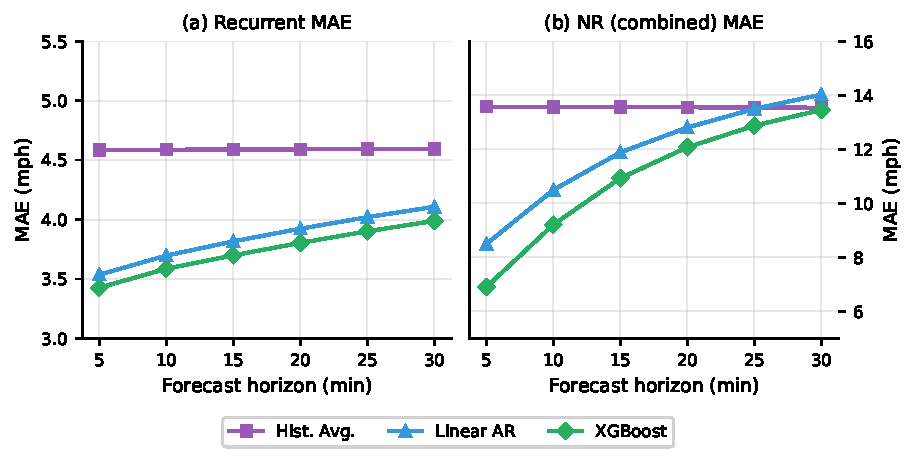
\includegraphics[width=\linewidth]{figures/horizon_mae.pdf}
  \caption{Per-horizon MAE on TSMO (\texttt{speed}/\texttt{standard})
           for three representative models.
           (a)~Recurrent MAE grows gradually with forecast horizon
           for all models.
           (b)~NR MAE (combined onset and confirmed NR) is consistently
           elevated and also grows with horizon.
           The historical average NR MAE is flat across horizons,
           reflecting that this model predicts a fixed reference
           regardless of recent speed dynamics; gradient-based models
           (Linear AR, XGBoost) benefit from short-horizon extrapolation
           but converge toward the historical average at 30~min.
           See Tables~\ref{tab:per_horizon_tsmo} and~\ref{tab:per_horizon_cranberry}.}
  \label{fig:horizon_mae}
\end{figure}

Tables~\ref{tab:per_horizon_tsmo} and~\ref{tab:per_horizon_cranberry}
report full per-horizon NR MAE for all 17 models on TSMO and Cranberry.
These repeat the h1--h6 columns from
Tables~\ref{tab:phase1_tsmo}--\ref{tab:phase1_cranberry}
in a standalone format for easier cross-model comparison.

\begin{table}[h]
\centering
\caption{Per-horizon NR MAE (mph) on TSMO,
         \texttt{speed}/\texttt{standard}.
         h1 = 5~min through h6 = 30~min.
         $\dagger$~D2STGNN values reflect an untrained model
         (see Appendix~\ref{app:exclusions}).}
\label{tab:per_horizon_tsmo}
\small
\begin{tabular}{lrrrrrr}
\toprule
Model & h1 & h2 & h3 & h4 & h5 & h6 \\
\midrule
Last Obs.          &  6.17 &  8.87 & 11.11 & 12.51 & 13.51 & 14.22 \\
Hist.\ Avg.        & 13.58 & 13.57 & 13.57 & 13.56 & 13.55 & 13.54 \\
Linear AR          &  8.57 & 10.60 & 12.03 & 12.98 & 13.71 & 14.28 \\
XGBoost            &  7.48 & 10.12 & 12.23 & 13.51 & 14.33 & 14.88 \\
\midrule
LSTM               &  6.57 &  8.87 & 10.67 & 11.88 & 12.74 & 13.37 \\
Transformer        &  6.54 &  8.89 & 10.71 & 11.97 & 12.86 & 13.52 \\
\midrule
HL                 &  6.17 &  8.87 & 11.11 & 12.51 & 13.51 & 14.22 \\
DGCRN              &  5.44 &  7.22 &  8.70 &  9.80 & 10.60 & 11.21 \\
GWNet              &  5.31 &  7.30 &  8.87 & 10.06 & 10.92 & 11.56 \\
STTN               &  5.28 &  7.36 &  8.97 & 10.17 & 11.04 & 11.67 \\
STGCN              &  5.79 &  7.57 &  9.09 & 10.23 & 11.07 & 11.70 \\
AGCRN              &  6.11 &  8.27 &  9.87 & 10.93 & 11.64 & 12.17 \\
DCRNN              &  5.94 &  8.02 &  9.66 & 10.90 & 11.83 & 12.52 \\

STGODE             &  5.75 &  7.99 &  9.79 & 11.17 & 12.17 & 12.93 \\
LSTM-ST            &  6.42 &  8.72 & 10.49 & 11.66 & 12.51 & 13.12 \\
ASTGCN             &  8.92 & 10.37 & 11.44 & 12.16 & 12.80 & 13.23 \\
D2STGNN$^\dagger$  & 17.44 & 17.65 & 18.04 & 17.35 & 17.89 & 18.15 \\
\bottomrule
\end{tabular}
\end{table}

\begin{table}[h]
\centering
\caption{Per-horizon NR MAE (mph) on Cranberry,
         \texttt{speed}/\texttt{standard}.
         h1 = 5~min through h6 = 30~min.
         $\dagger$~D2STGNN anomaly discussed in
         Section~\ref{sec:finding3}.}
\label{tab:per_horizon_cranberry}
\small
\begin{tabular}{lrrrrrr}
\toprule
Model & h1 & h2 & h3 & h4 & h5 & h6 \\
\midrule
Last Obs.          &  6.83 &  8.16 &  9.08 &  9.50 &  9.75 &  9.94 \\
Hist.\ Avg.        & 12.03 & 12.00 & 11.97 & 11.95 & 11.94 & 11.92 \\
Linear AR          &  6.79 &  7.59 &  8.02 &  8.28 &  8.47 &  8.65 \\
XGBoost            &  6.35 &  7.22 &  7.73 &  8.06 &  8.30 &  8.48 \\
\midrule
LSTM               &  6.21 &  7.09 &  7.64 &  8.01 &  8.27 &  8.51 \\
Transformer        &  6.27 &  7.07 &  7.59 &  7.94 &  8.20 &  8.44 \\
\midrule
HL                 &  6.83 &  8.16 &  9.08 &  9.50 &  9.75 &  9.94 \\
DGCRN              &  5.65 &  6.55 &  7.06 &  7.44 &  7.74 &  7.99 \\
GWNet              &  5.61 &  6.54 &  7.10 &  7.49 &  7.81 &  8.05 \\
STTN               &  5.67 &  6.69 &  7.22 &  7.59 &  7.94 &  8.19 \\
STGCN              &  5.92 &  6.76 &  7.26 &  7.62 &  7.92 &  8.19 \\
AGCRN              &  5.96 &  6.82 &  7.33 &  7.68 &  7.95 &  8.19 \\
DCRNN              &  5.82 &  6.78 &  7.36 &  7.82 &  8.21 &  8.57 \\
STGODE             &  6.01 &  6.86 &  7.41 &  7.79 &  8.09 &  8.35 \\
LSTM-ST            &  6.22 &  7.06 &  7.58 &  7.93 &  8.19 &  8.44 \\
ASTGCN             &  7.95 &  8.27 &  8.49 &  8.67 &  8.81 &  8.96 \\

D2STGNN$^\dagger$  & 12.06 & 12.14 & 12.36 & 11.97 & 12.22 & 12.42 \\
\bottomrule
\end{tabular}
\end{table}

% ══════════════════════════════════════════════════════════════
\section{Network and NR Episode Statistics}
\label{app:data_stats}
% ══════════════════════════════════════════════════════════════

Table~\ref{tab:network_stats} summarizes key properties of the two
study networks and their NR episode distributions.

\begin{table}[h]
\centering
\caption{Network and NR episode statistics for the study datasets.}
\label{tab:network_stats}
\small
\begin{tabular}{lrr}
\toprule
Property & TSMO & Cranberry \\
\midrule
Links ($N$)                          & 228 & 78 \\
Observation period                   & Feb 2022--Feb 2023 & Feb 2022--Jan 2024 \\
Total timesteps ($T$)                & 48,360 & 97,092 \\
Sessions (weekday operating days)    & 260 & 522 \\
Temporal resolution                  & 5 min & 5 min \\
Operating hours                      & 05:30--20:55 & 05:30--20:55 \\
\midrule
NR rate (full period, \%)            & 3.97 & 2.42 \\
NR rate (train split, \%)            & 3.92 & 2.32 \\
NR rate (val split, \%)              & 5.12 & 2.98 \\
NR rate (test split, \%)             & 3.01 & 2.31 \\
\midrule
Weather features ($W$)               & 18 & 12 \\
Min.\ confirmation window            & 3 steps (15 min) & 3 steps (15 min) \\
\midrule
Train windows                        & 31,304 & 62,840 \\
Val windows                          & 6,708 & 13,458 \\
Test windows                         & 6,708 & 13,458 \\
\bottomrule
\end{tabular}
\end{table}

The NR rate in the validation split is notably higher than in train
and test splits on both networks (TSMO: 5.12\% vs.\ 3.92/3.01\%;
Cranberry: 2.98\% vs.\ 2.32/2.31\%).
This imbalance is an artefact of the chronological split: both
networks experience elevated NR activity in their respective
mid-year periods, which fall predominantly in the validation split.
The elevated validation NR rate benefits the early-stopping criterion
(monitored on validation NR~MAE) but does not affect the test results.

% ══════════════════════════════════════════════════════════════
\section{Hyperparameter Tuning for NR-Aware Strategies}
\label{app:hyperparams}
% ══════════════════════════════════════════════════════════════

The three NR-aware training strategies introduce additional
hyperparameters tuned on the TSMO validation set NR~MAE:

\begin{itemize}
  \item \textbf{Weighted loss} ($\lambda$):
        upweighting factor for confirmed NR steps.
        Grid: $\{2, 5, 10, 20\}$.
        Selected: $\lambda = 5$.
  \item \textbf{NR fine-tune} ($\mu$):
        learning rate multiplier for phase~2 fine-tuning.
        Grid: $\{0.05, 0.1, 0.2\}$.
        Selected: $\mu = 0.1$.
  \item \textbf{Multi-objective} ($\gamma$):
        weight of BCE auxiliary loss relative to speed MSE.
        Default: $\gamma = 1.0$ (equal weighting);
        not tuned separately as the auxiliary loss scale is
        calibrated by the linear head initialization.
\end{itemize}

Tuning was performed on the LSTM model on TSMO with the
\texttt{speed} feature configuration and applied unchanged to
all models and to Cranberry.
The selected $\lambda = 5$ and $\mu = 0.1$ represent moderate
NR emphasis: stronger upweighting ($\lambda = 20$) improves
NR~MAE marginally but degrades recurrent~MAE substantially.

%%─────────────────────────────────────────────────────────────
%% References
%%─────────────────────────────────────────────────────────────

\bibliographystyle{elsarticle-harv}
\bibliography{paper}


\end{document}
